% \Image{Capa do livro (; )}{PNLD2022-024-01.png}
% \Image{Foto do autor e ilustrador (Arquivo pessoal; )}{PNLD2022-024-02.png}
% \Image{Ilustração do livro (; )}{PNLD2022-024-04.png}
% \Image{Ilustração do livro (; )}{PNLD2022-024-05.png}
% \Image{Ilustração do livro (; )}{PNLD2022-024-06.png}




\documentclass[11pt]{extarticle}
\usepackage{manualdoprofessor}
\usepackage{fichatecnica}
\usepackage{lipsum,media9}
\usepackage[justification=raggedright]{caption}
\usepackage[one]{bncc}
\usepackage[maisemelhores]{../edlab}
\usepackage{marginnote}
\usepackage{pdfpages}
\usepackage[printwatermark]{xwatermark}
%\newwatermark[pagex=2]{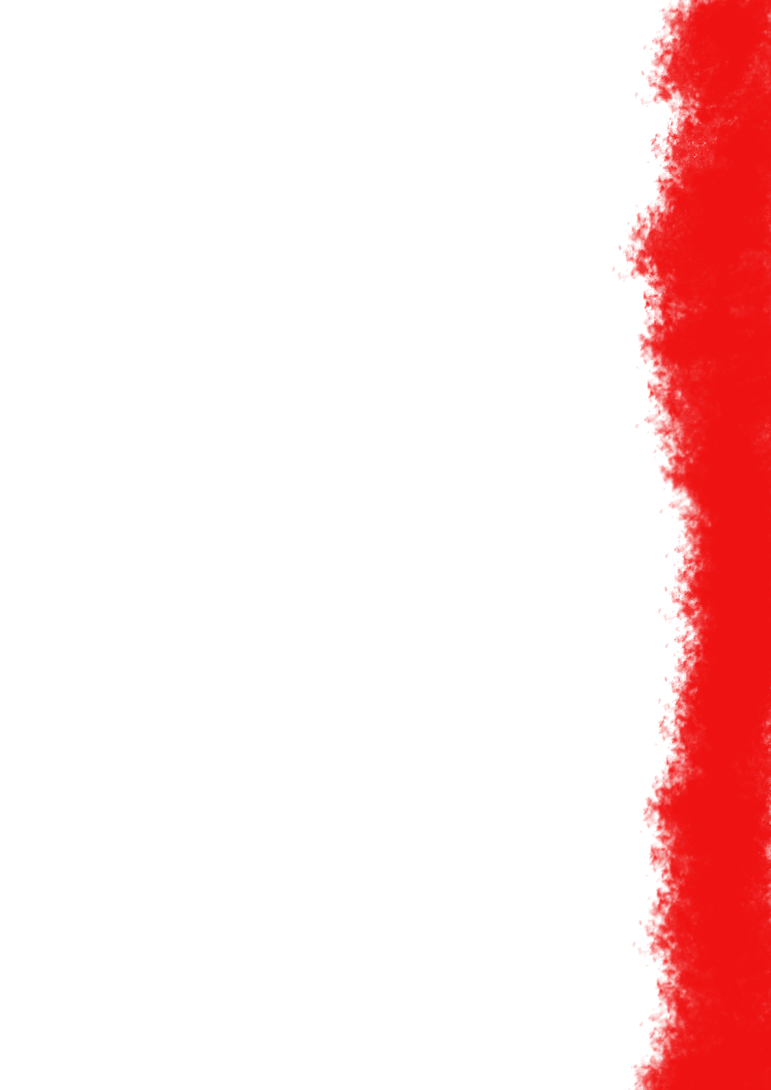
\includegraphics[scale=3.3]{watermarks/test-a.png}}	% página específica
%\newwatermark[oddpages]{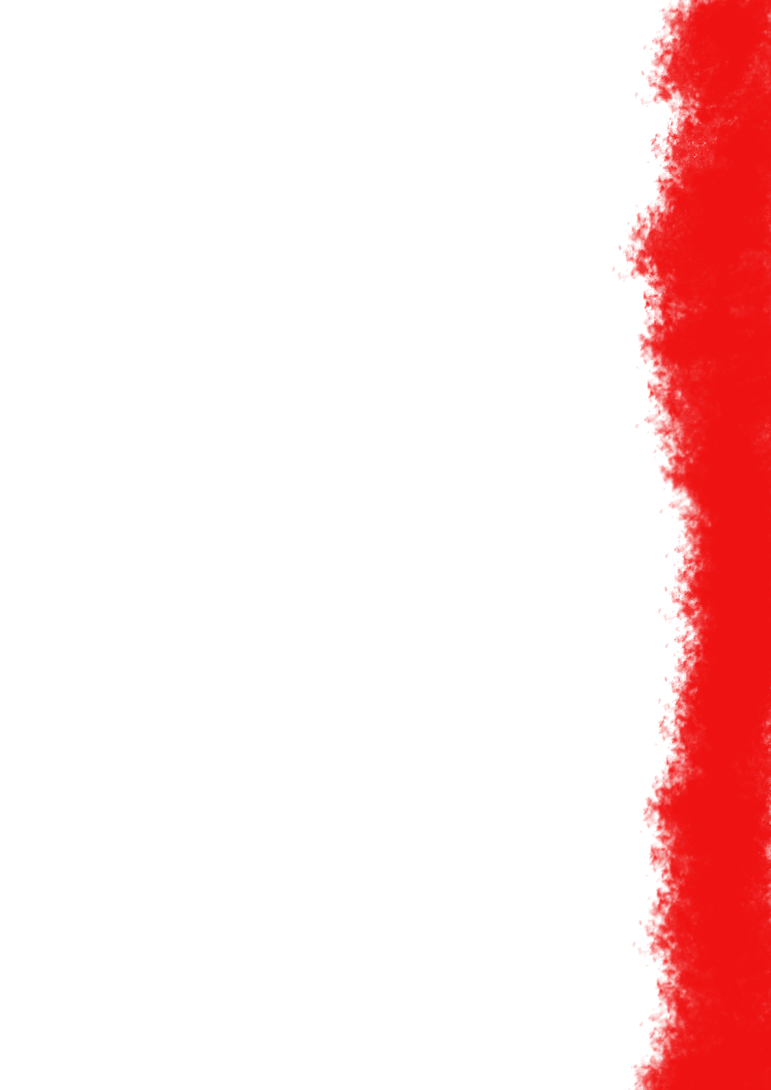
\includegraphics{watermarks/test-a.png}}			% páginas ímpars
%\newwatermark[evenpages]{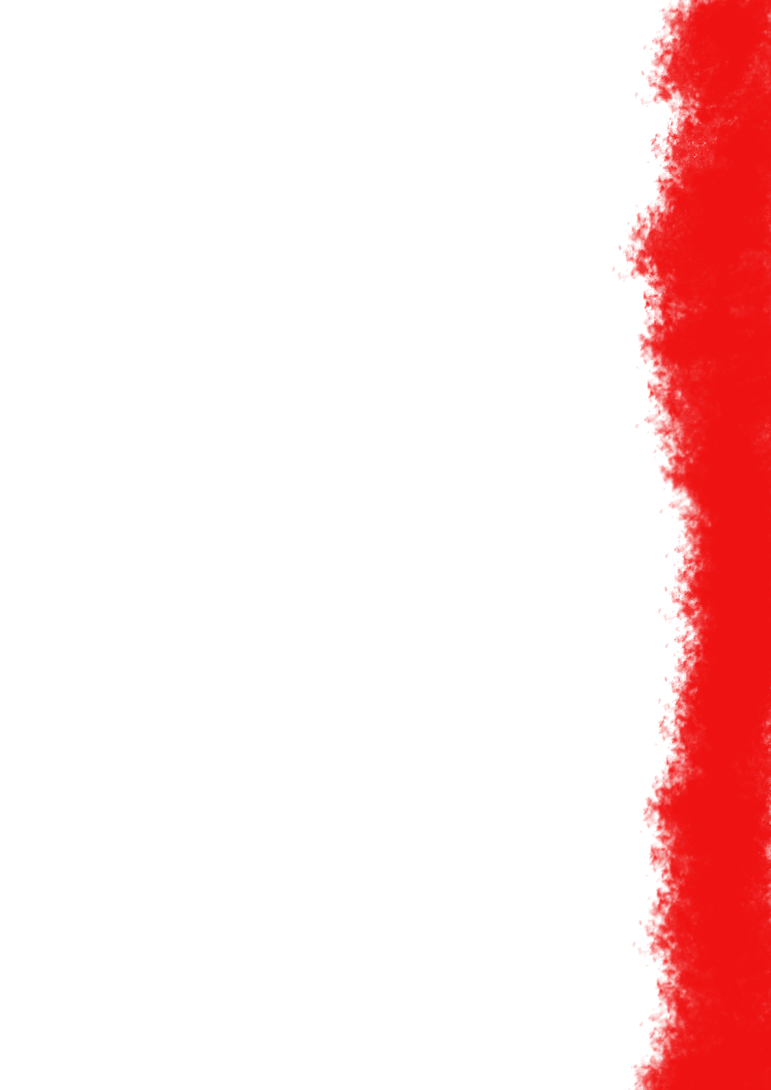
\includegraphics{watermarks/test-a.png}}			% págimas pares
\newwatermark[allpages]{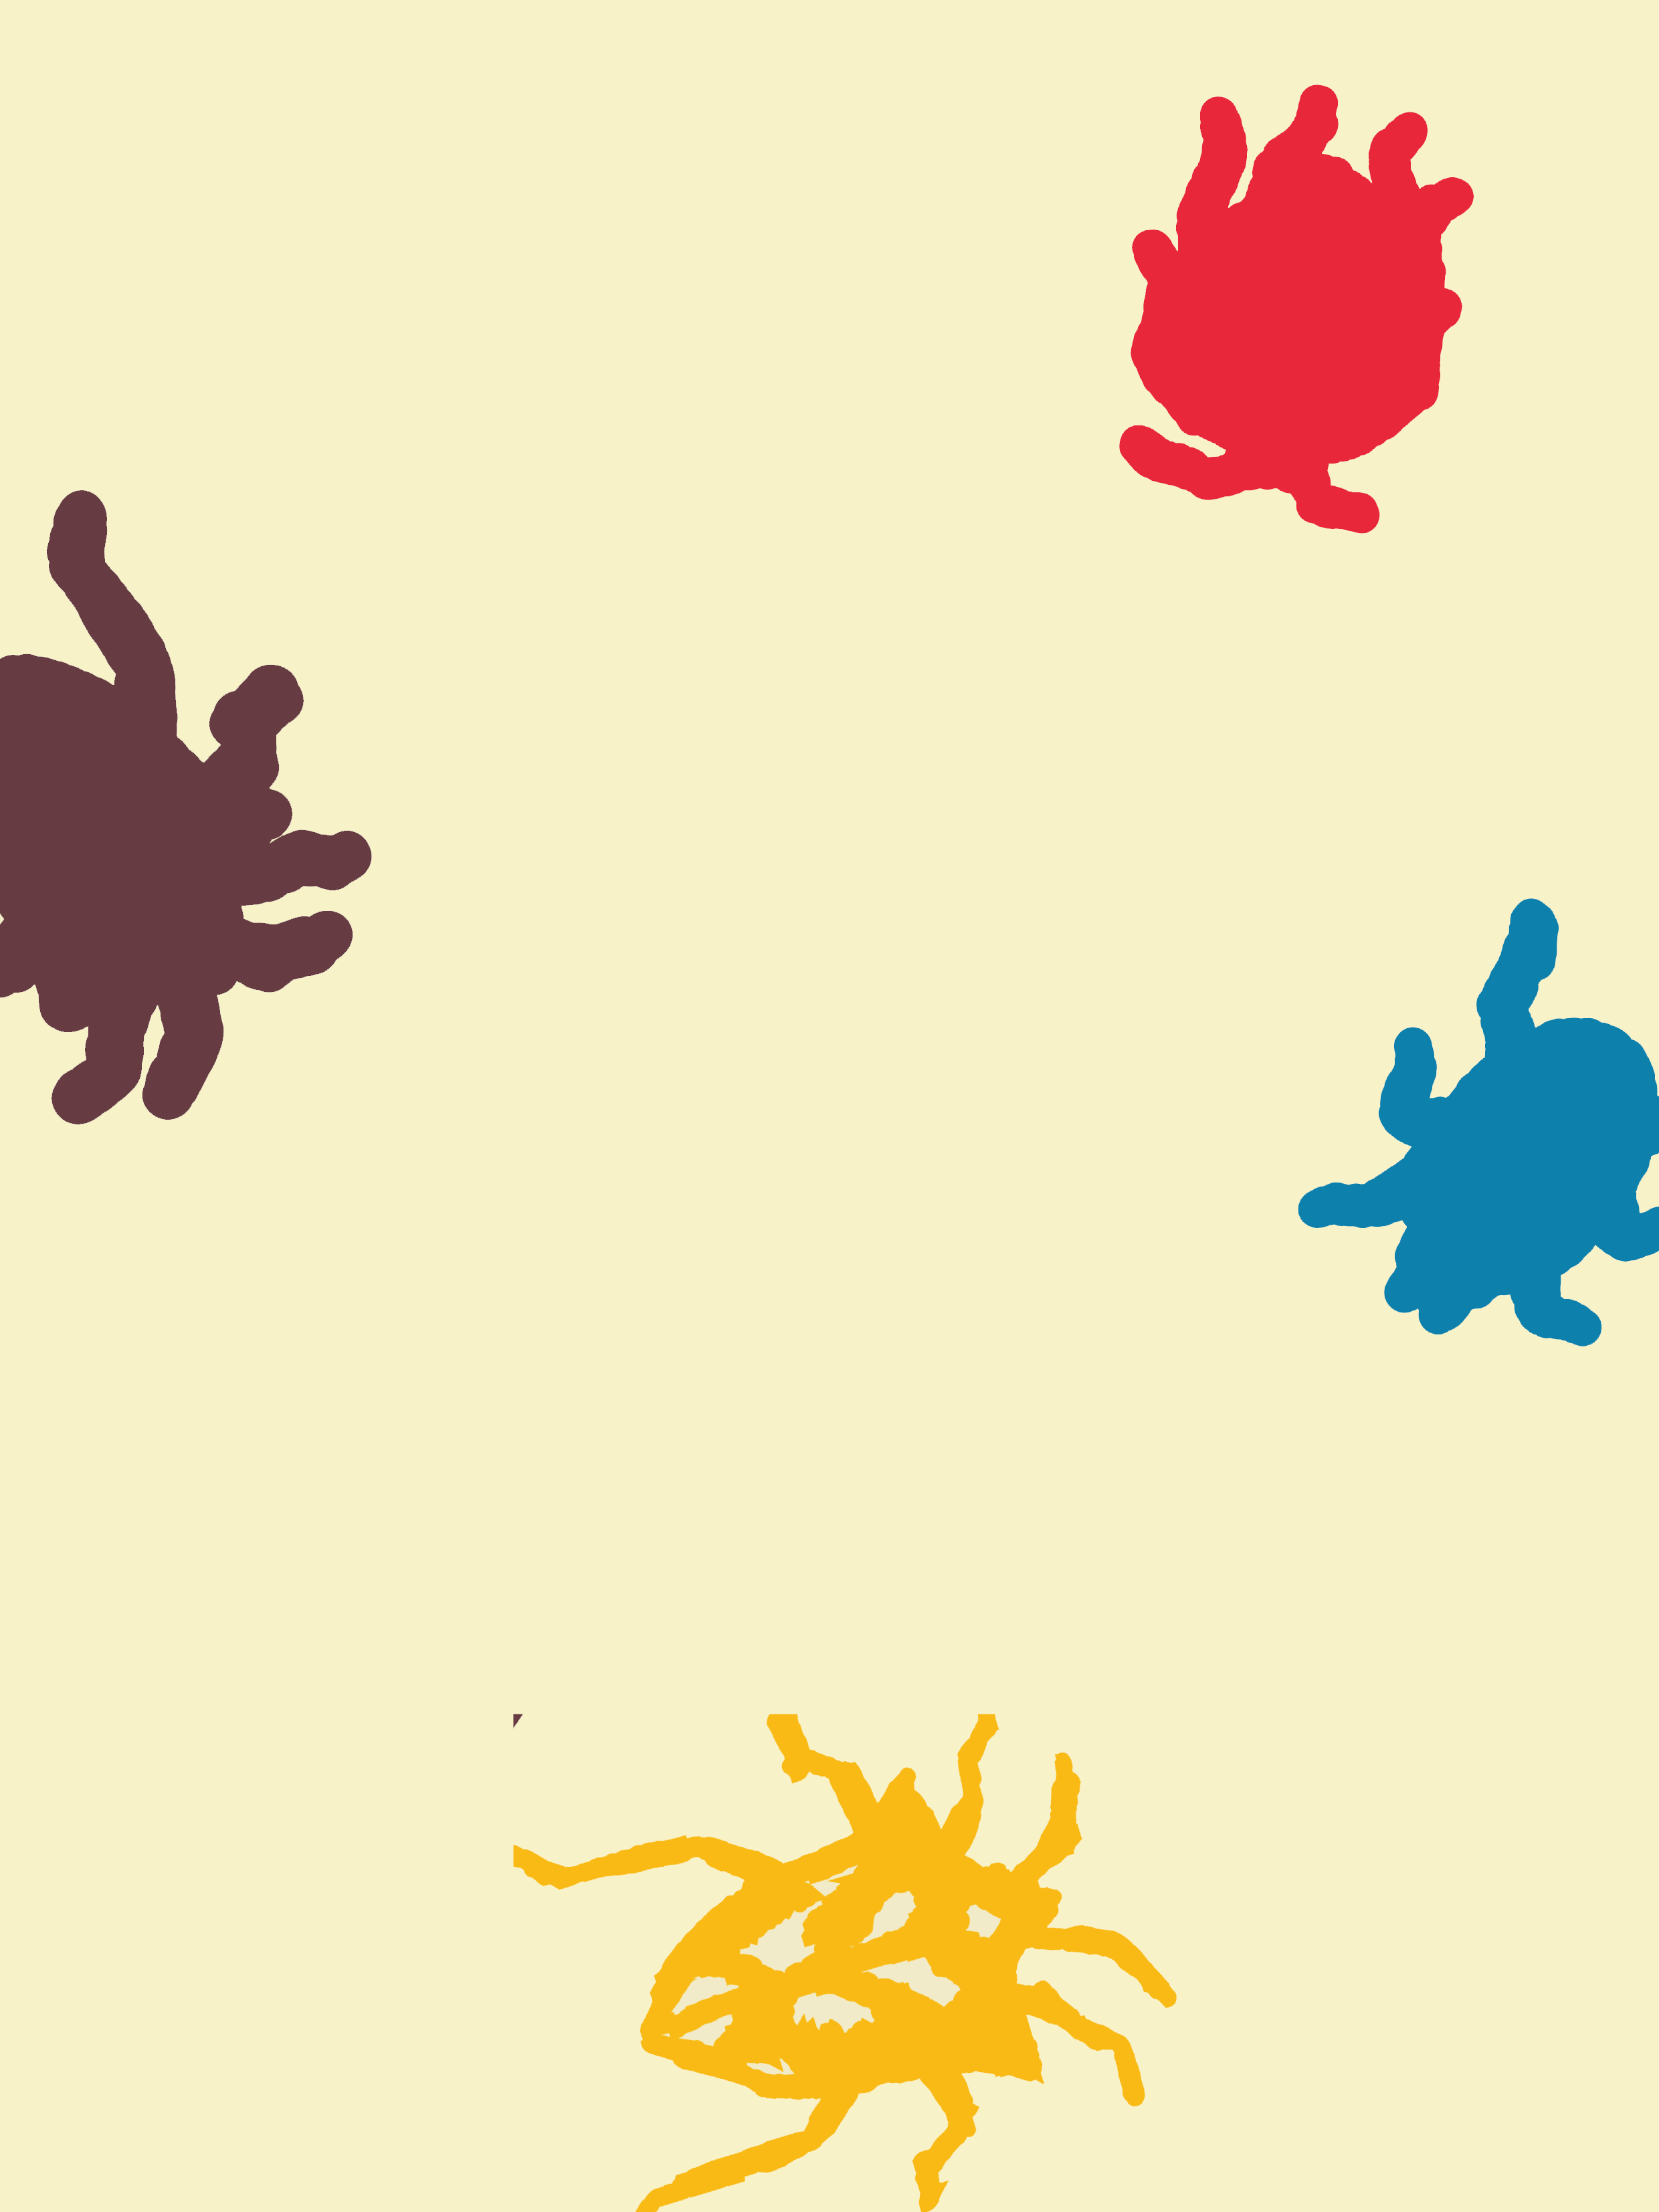
\includegraphics[scale=1]{watermarks/024.png}}

\pagecolor{cyan!0!magenta!10!yellow!28!black!28!}

\newcommand{\AutorLivro}{Lucas-K}
\newcommand{\TituloLivro}{Fim dos insetos}
\newcommand{\Tema}{Mundo natural; meio ambiente; plantas; Biologia e Ciências}
\newcommand{\Genero}{Narrativos: fábulas originais; da literatura universal e da tradição popular; etc}
\newcommand{\imagemCapa}{./images/PNLD2022-024-01.png}
\newcommand{\issnppub}{978-65-99442-24-7}
\newcommand{\issnepub}{978-65-99442-26-1}
% \newcommand{\fichacatalografica}{PNLD0001-00.png}
\newcommand{\colaborador}{{Paulo Pompermaier e Renier Silva}}

\begin{document}

\title{\TituloLivro}
\author{\AutorLivro}
\def\authornotes{\colaborador}

\date{}
\maketitle

%\begin{abstract}\addcontentsline{toc}{section}{Carta ao professor}
%\pagebreak

\tableofcontents



\section{Sobre o livro}

%27 caracteres
\paragraph{O livro} \textit{Fim dos insetos}, de Lucas-K, é uma envolvente narrativa sobre a interação entre insetos e humanos na Terra. Vários insetos são retratados de forma lúdica e colorida --- a cigarra, a joaninha, o mosquito, o carrapato, o pulgão ---, em seu dia a dia nas cidades. No entanto, um problema com os humanos, que não conseguiam entender e conviver com os pequenos bichinhos, levou os insetos a deixarem as cidades e se unirem nas floresta. Depois disso, as cidades nunca mais seriam as mesmas: perderam o colorido da diversidade de vida, inclusive as flores, que não nasceram mais quando deixaram de ser polinizadas pelos insetos.

%822 caracteres
\paragraph{Descrição} Muitos insetos viviam nas cidades. Nem todos eram bonitos como as joaninhas, mas todos tinham suas funções, mesmo as baratas que visitavam as lixeiras durante a noite. As pessoas, por isso, começaram a ter medo deles, e muitos eram esmagados. Nem a bela joaninha conseguiu fugir dessa sorte: Clarice, a única humana nomeada na história, assustou-se certa vez com um bichinho na parede e, sem querer, jogou veneno em uma pobre joaninha. Os insetos, tristes, resolveram mudar a situação. O pulgão reuniu todos os insetos para conversar e procurar uma solução. O mosquito queria picar todos os humanos, mas resolveram que a melhor solução não era machucar as pessoas. Incentivados pelo bicho-folha, formaram uma grande fila e foram morar na floresta. Na cidade, no entanto, sentiram sua falta, pois as flores não mais nasciam e parecia faltar alguma coisa no ciclo da vida.


%411 caracteres
\paragraph{Competências} 
Com este livro, as crianças da \textbf{Pré-escola} poderão
trabalhar competências que dizem respeito ao conhecimento dos
insetos da fauna local, sua importância para o funcionamento do ecossistema e o respeito à biodiversidade. Além de conhecer os insetos, as crianças também vão explorar o universo das cores, pois cada página é ilustrada com uma diversidade delas. O enrendo da história, ainda, mobiliza competências relacionadas à interação da criança com o mundo, pois fala sobre o valor da diferença e a importância de respeitar aquilo que não compreendemos, pois tudo tem uma função no mundo.

%862 caracteres
\paragraph{Aprofundamento} 
Este material tem a intenção de contribuir para que você consiga desenvolver um trabalho aprofundado 
com esta obra na sala de aula. Você encontrará informações sobre o autor, sobre 
o gênero e sobre os temas trabalhados ao longo do livro. Apresentaremos também 
algumas propostas de trabalho para a sala de aula que você poderá explorar livremente, 
da forma que considerar mais apropriada para os seus estudantes. Para a prática 
da Literacia Familiar, oferecemos um guia que pode ajudar nas orientações aos 
responsáveis pela criança, para incentivar o gosto pela leitura e contribuir para 
que os estudantes desenvolvam em casa habilidades que serão importantes no momento 
da alfabetização. Por fim, você encontrará sugestões de livros, artigos e sites 
selecionados para enriquecer a sua experiência de leitura e, 
consequentemente, a de seus estudantes.


\section{Sobre o autor}

%532 caracteres
\paragraph{O autor} Lucas-K, nome artístico de Lucas de Mesquita Kröeff, é um artista visual brasileiro. Bacharel em Design pela Universidade Federal de Minas Gerais (\textsc{ufmg}) e em Artes Visuais pela Cambridge School of Arts (Ruskin School), na Inglaterra, desenvolve seus trabalhos numa interface livre entre iniciativas independentes, instituições de arte e editoras de livros, produzindo instalações, livros, vídeos e experiências coletivas.
Lucas Kröeff explora, em seus trabalhos, a relação entre história, política, imaginação coletiva e a construção da sua própria subjetividade, num processo de construção de redes de intercâmbio, assim como de procedimentos sistemáticos de organização da vida quotidiana.

%313 caracteres
\paragraph{Publicações} Como artista gráfico, Lucas Kröeff desenvolve capas de livros e coleções de livros usando o alfabeto como ferramenta de desenho conceitual. Ele já fez capas de livros de autores como Masha Alyokhina, Félix Guattari, Harriet Jacobs, Walter Benjamim, Franz Kafka, Fernando Pessoa, Celso Favaretto, Paul D. Escott, Baudelaire, Maquiavel, H.P. Lovecraft, Fernand Deligny, Stéphane Mallarmé e outros.

%358 caracteres
\paragraph{Currículo} Lucas Kröeff já teve trabalhos apresentados na 11ª Bienal de Arquitetura de São Paulo, Museu de Tecnologia de Cambridge, Cinemateca de São Paulo, Museu de Minas e Metal, \textsc{iiix} Festival Internacional de Videoarte de Barcelona e ARCOMadrid, entre outras instituições e galerias de arte. Em 2015 recebeu o Prêmio de Arte da Sustentabilidade em Cambridge (Reino Unido). Publica livros há mais de 10 anos.
Foi co-fundador e participou em vários coletivos de arte, incluindo a Atpress em Londres, bem como nos grupos \textsc{mapa}, \textsc{banca} e Quadradocirculo no Brasil.


\section{Sobre o gênero}

%55 caracteres
\paragraph{O gênero} O gênero deste livro é \textit{narrativa}. 

%596 caracteres
\paragraph{Descrição} 
O gênero narrativo possui uma variedade de tipos e, cada um, suas estruturas específicas.
A característica comum entre todos é que sempre há uma história a ser contada, com linearidade,
ou seja, começo, meio e fim, e personagens. 
Dentre os tipos de narrativas mais comuns na literatura infantil, estão: mito, lenda, 
fábula e apólogo. Este último, semelhante à fábula, possui personagens não humanos, 
dramatização de fala, e uma moral, implícita ou explícita, mas difere na natureza destas 
personagens: se no caso da fábula se trata de animais, no caso do apólogo as personagens 
são objetos inanimados. A narrativa deste livro poderia ser classificada como uma fábula, pois dá subjetividade aos insetos e explora suas relações, com diálogos entre eles e a procura de soluções em grupo. Quase qualquer coisa pode ser uma personagem de uma narrativa 
infantil, já que a capacidade reflexiva das crianças nesta idade ainda está em um nível primário. 


%603 caracteres
\paragraph{Interação} 
As narrativas são uma forma de inserir os sujeitos no mundo. 
São elas que apresentam boa parte dos valores culturais da sociedade 
onde se vive. Mas não é só passivo o papel das crianças nesta experiência. 
As interações entre dois ou mais personagens onde se verifica
uma ação de linguagem organiza e impulsiona experiências compartilhadas,
importantes para o desenvolvimento psíquico do sujeito nos primeiros anos de vida.
Neste sentido, as narrativas são uma ótima ferramenta para
apresentar o mundo e capacitar as crianças para viver nele, mas como se
trata de um trabalho com a linguagem, sempre dando espaço à individualidade, 
seja na compreensão das histórias, na identificação com as personagens, ou 
no ato de narrar. 

%862 caracteres
\paragraph{Competências} 
Através de elementos dos mitos, contos e histórias do cotidiano, desenvolve-se a sensibilidade narrativa e a capacidade de imaginação das crianças. Para um bom desenvolvimento da capacidade narrativa e imaginativa é necessária a intermediação do educador, que vai trazer novos olhares, análises e discussões para ajudar a criança na construção do significado. Essas são etapas fundamentais para o desenvolvimento linguístico e a aquisição das competências de leitura e escrita. Por meio da narrativa, inclusive, a criança passa do diálogo ao monólogo, pois passa a ser capaz de elaborar um discurso para si com maior autonomia, sem a intermediação necessária no diálogo.
O conjunto de elementos verbais e visuais da narrativa proporcionam, assim,
uma abertura ao mundo e um convite para integrá-lo pela curiosidade e pela imaginação.

\Image{O gênero da narrativa proporciona ao leitor uma abertura ao mundo. (Pixabay/Tumisu; CC-BY-2.0)}{PNLD2022-024-07.png}

A narrativa de \textit{Fim dos insetos}, em especial, trabalha diferentes competências
nos pequenos leitores. Para além da narrativa, o livro apresenta às crianças uma linguagem artística complexa.
Explorar as cores, as formas, o posicionamento das personagens 
na página e até mesmo a opinião e os sentimentos das crianças sobre as imagens e a narrativa
são possibilidades que aprofundarão a leitura, aumentarão o repertório 
e incentivarão o desenvolvimento do vocabulário e da fluidez do discurso. 


\section{Temas}

\subsection{Mundo natural; meio ambiente; plantas; Biologia e Ciências}

%136 caracteres
\paragraph{Abordagem} Os protagonistas desta história são os insetos, e o enrendo é todo estruturado na sua importância para o meio ambiente e para a preservação do ecossistema e manutenção do mundo natural.

 
%206 caracteres
\paragraph{Descrição} O tema do mundo natural e do meio ambiente é estruturado, nesta narrativa, na vida dos insetos. Diversas espécies são apresentadas: besouro, pulgão, cigarra, joaninha, mosquito, carrapato, bicho-folha, barata etc. Apesar do conflito com os humanos, gradualmente percebe-se a importância dos bichinhos para a manutenção do meio ambiente, introduzindo à criança conceitos fundamentais às ciências biológicas como cadeia alimentar, ecossistema e ciclo de vida.

%275 caracteres
\paragraph{Competências} 
A associação entre o cantar do galo e o nascer do dia é intrínseca
à cultura brasileira. Sobretudo na área rural, onde estes bichos
existem em maior quantidade. Tanto para as crianças que vivem
esta realidade quanto para aquelas que só vêm os galos em desenhos
animados, por exemplo, o quotidiano do galo Gogó é importante 
pois ensina elementos essenciais dos hábitos sociais. Acordar cedo com
o sol, dormir à noite e sonhar. 

\section{Modelagem de aula}
A seguir você encontrará a descrição de uma aula modelo como exemplo 
prático de exploração do livro com estudantes. Esta seção apresentará 
orientações sobre como organizar a sala de aula para receber os 
estudantes, exercitar a interação verbal e prepará-los para o 
momento da leitura.

Em seguida, você encontrará a \textbf{Leitura dialogada}, um 
tópico destinado a te orientar para o momento específico da 
leitura com os estudantes. Por fim, no tópico 
\textbf{Propostas de atividades}, você encontrará ideias 
de práticas que pode explorar com as crianças em sala de 
aula após a leitura. 

Essas atividades podem ser trabalhadas de acordo com a 
disponibilidade do seu cronograma e fique à vontade para adaptá-las 
da forma que achar melhor para os seus estudantes. Cada turma é única 
e o seu conhecimento prático das características de cada aluno será 
essencial para definir a melhor forma de aplicar essas ideias. 

O objetivo deste manual é oferecer algumas ideias 
e inspirações para um trabalho que pode ser desenvolvido tanto 
a curto, quanto a médio e longo prazo. Sinta-se a vontade para 
personalizar a aula e torna-la sua, aplicando seus conhecimentos, sua 
personalidade e aproveite para fortalecer 
seu vínculo com a turma.


\subsection{Antes de ler}

\BNCC{EI03EF01}
\BNCC{EI03ET01}
\BNCC{EI03ET03}
\BNCC{EI03ET05}
\BNCC{EI03EO01}
\BNCC{EI03EO03}
\BNCC{EI03EO04}

%Alterar o nível escolar nesse parágrafo.
Como este trabalho será realizado com crianças da \textbf{Pré-escola}, 
que ainda não têm muita intimidade com o livro enquanto objeto, você terá o 
papel de mediar este contato. 

Nosso objetivo é que os próprios estudantes possam manusear 
e explorar o livro de forma autônoma, mas, para que isto aconteça, você 
pode ajudar a tornar o caminho mais convidativo com atividades que tenham 
intencionalidade educativa. 

A \textsc{bncc} define intencionalidade educativa como ``organização 
e proposição, pelo educador, de experiências que permitam às crianças 
conhecer a si e ao outro e de conhecer e compreender as relações com a 
natureza, com a cultura e com a produção científica, que se traduzem nas 
práticas de cuidados pessoais (alimentar-se, vestir-se, higienizar-se), 
nas brincadeiras, nas experimentações com materiais 
variados, na aproximação com a literatura e no encontro com as 
pessoas''.\footnote{\textsc{bncc}, página 39}

É importante manter essa intencionalidade em mente não apenas na condução 
das atividades propostas neste manual, mas também para aproveitar as 
oportunidades espontâneas de construir conhecimentos que podem surgir durante 
a interação direta com os estudantes.

\begin{enumerate}
%836 caracteres
\item \textbf{O ambiente}\quad Antes de iniciar o trabalho com o livro, é importante que você prepare o ambiente para receber a turma. Como o trabalho com o livro terá 
três momentos (antes, durante e depois da leitura), seria interessante que você 
criasse um ambiente para cada etapa. Nas \textbf{Sugestões de referências complementares} 
você encontrará um artigo que discorre sobre a importância da organização da sala 
de aula para a educação infantil, que pode ser um bom guia para a criação desses 
ambientes. Para o momento antes da leitura, sugerimos uma atividade que envolve a família e estimule a percepção da criança sobre os insetos em seu cotidiano.
Será necessário comunicar os pais com antecedência para que, junto à criança, tentem tirar uma fotografia de um inseto em seu quotidiano. Posteriormente, os pais devem enviar a fotografia ao professor. Na impossibilidade de realizar a fotografia, pode-se pedir aos pais que realizem outra tarefa com a criança para representar o inseto: um desenho, um pequeno texto etc. A atividade pode ser desenvolvida em sala de aula ou, preferencialmente, em um local aberto, para possibilitar a observação da natureza e a interação com o mundo natural, tão presente no livro.

%632 caracteres
\item \textbf{Desenvolvimento}\quad O professor explicará, com uma semana de antecedência, que os alunos devem tirar a fotografia de um inseto com seus pais e enviar a foto ao professor. No dia da atividade, o educador pode imprimir as fotos para mostrar para a turma ou projetá-las em uma sala de vídeo. Na impossibilidade de realizar a atividade com os pais, o professor pode selecionar algumas fotos da internet de insetos comuns ao quotidiano (abelhas, formigas, besouros, baratas, mosquitos etc.) e apresentá-las ao alunos.
Em uma primeira aproximação, o professor pode perguntar aos alunos o que observam de diferente entre os insetos: os diferentes tamanhos, formas, cores, antenas, patas etc. Explore a percepção das diferenças entre as crianças.
Depois, relacione as fotografias à experiência dos alunos: pergunte quem conhece aqueles insetos, quem já os viu em sua casa ou em seus arredores, o que sentiram, se tiveram medo etc. Se foi possível realizar a foto com os pais, pode-se explorar ainda mais essa interação, perguntando aos estudantes como foi o momento da foto, onde encontraram o inseto, o que sentiram etc.
Facilite a comunicação entre as crianças mediando os diálogos e fomentando-os a trocar informações sobre as características dos insetos.

\Image{Exemplo de ilustração de insetos a ser apresentada na sala de aula. (Adolphe Millot/Public domain pictures; Domínio público)}{PNLD2022-024-09.png}

\item \textbf{Perguntas para avaliar}\quad As crianças interagiram e se interessaram pelas fotografias? Conseguiram perceber as diferenças? E as semelhanças? Elas já conseguem diferenciar cores, formas, tamanho? Se não, como estimular a aquisição dessas habilidades? 
\end{enumerate}


\subsubsection{A interação verbal} 
Criar situações em que as crianças precisam dialogar diretamente com 
você é uma das práticas mais importantes de Literacia, pois elas estimulam 
o desenvolvimento linguístico, ampliam o vocabulário e reforçam a 
capacidade dos estudantes de compreenderem o que ouvem e se expressarem 
pela fala. O diálogo livre com a criança também reforça sua autoestima, pois 
a faz se sentir ouvida e valorizada pelo adulto, ao vê-lo prestar atenção 
no que ela tem a dizer. Portanto, sempre que possível, reserve um tempo na 
aula apenas para a interação verbal. 

Como esse tipo de interação é espontânea e intimamente atrelada ao 
desenvolvimento de cada estudante, nossas orientações não serão específicas. 
A ideia é que você adapte este momento de acordo com as respostas e os 
repertórios das crianças. É um momento de estreitamento de vínculos e, portanto, 
fique à vontade para ser espontânea e para explorar os tópicos que achar 
mais interessantes para a sua turma.

Inicie as conversas com naturalidade, seguindo os objetos de atenção das crianças. 
Você pode partir de objetos que estejam analisando
para iniciar um assunto e incentivar que se expressem. Ainda que a
criança não fale corretamente, continue interagindo, 
pois a intenção aqui é que a criança perceba que outras pessoas estão respondendo 
à sua comunicação. 

Fique atento a todas as formas de expressão: os gestos, as falas, as 
expressões faciais, para onde olham\ldots{} tudo pode ser explorado durante a conversa. 
Demonstre curiosidade sobre eles, seja um ouvinte entusiasmado e incentive que eles 
conversem entre si. Faça perguntas e construa a resposta junto com as crianças. 

A seguir, algumas dicas que podem contribuir para que a interação verbal 
seja produtiva em sua sala de aula: 

\begin{enumerate}
\item Sente-se no chão e brinque com eles, estabelecendo 
contato visual. Além das pequenas frases que conseguem formar, vocalizações, 
gestos e expressões faciais podem ser boas formas de comunicar.

\item Não se esqueça que a conversa é uma troca e, portanto, 
evite ficar falando sozinho ou desvalorizar as respostas das 
crianças quando não conseguem formular frases completamente articuladas. 
Nunca descarte uma tentativa de comunicação. 

\item Evite utilizar falas negativas que desencorajam o diálogo. 
Se precisar que a turma 
corrija algum comportamento, explique claramente a razão e 
oriente com calma. Incentive positivamente as crianças e 
destaque o motivo de seus elogios. 

\item Aproveite alguns momentos durante a conversa para chamar 
a atenção das crianças para os sons das palavras e das letras que você 
acabou de usar ou que eles pronunciaram.  

\item Fale sempre com as crianças, pois, apesar de alguns estarem começando a falar,
são capazes de compreender muito.

\item Explore possibilidades de interação como apontar e 
nomear objetos, pessoas e animais, imitar a criança ou pedir que 
ela o imite, fazer caretas, reproduzir sons de 
animais para que repitam, ensinar os nomes de partes do corpo, 
entre outras atitudes que estimulem a comunicação com a criança. 

\item Muitas dessas dicas poderão ser aproveitadas pela 
família durante a prática da Literacia Familiar. Portanto, 
se achar necessário, compartilhe algumas destas orientações 
com as famílias dos estudantes.
\end{enumerate}


\subsection{A leitura dialogada}
Este é o momento em que será realizada a leitura propriamente dita. 
Se possível, crie um \textit{cantinho da leitura} em sua sala de aula. Um 
ambiente confortável, de preferência em que todos se sentem no chão ou 
em pufes para que consigam enxergar as ilustrações do livro que está 
sendo lido e interagir com facilidade. Se houver possibilidade, mantenha 
sempre os livros da turma em uma altura da estante que permita fácil 
acesso para os estudantes ou guarde os livros em uma caixa que as crianças 
possam mexer com autonomia. É importante que elas tenham autonomia para 
acessar os livros e se sintam à vontade para pegá-los sempre que quiserem. 

\Image{É importante que o cantinho da leitura proporcione autonomia para as crianças. (Elza Fiúza/ Agência Brasil; CC BY-NC 2.0)}{PNLD2022-024-08.png}

Outra possibilidade de ambiente para esta leitura, se a escola permitir, 
é efetuar essa leitura ao ar livre, embaixo de uma árvore, onde as crianças 
possam ouvir os sons dos pássaros e sentir o cheiro da grama. Sair da sala 
de aula pode oferecer um ótimo leque de experiências aos seus estudantes e 
reforçar a conexão entre a natureza do livro e a realidade.  

Reserve uma boa parte da aula para o momento da leitura com os estudantes, 
pois é importante que esse momento aconteça sem pressa. O objetivo da 
leitura dialogada é que seja uma leitura em bate-papo. A criança deve 
assumir um papel ativo na leitura, mesmo que ainda não seja capaz de 
ler sozinha. Além de promover o gosto pela leitura, esta prática estimula 
o desenvolvimento da linguagem, enriquece o vocabulário e 
aumenta o conhecimento de mundo.

%Especificar o livro.
No caso de \textit{Fim dos insetos}, o diálogo durante a leitura é 
importante para que as crianças deem atenção aos detalhes
do texto escrito e às ilustrações.
Você deve interagir com eles durante toda a 
leitura, fazendo perguntas e partindo de detalhes do livro para 
levantar novas questões. 

A seguir, algumas orientações para aproveitar este momento: 

\begin{enumerate}
%177 caracteres
\item \textbf{Como começar}\quad Sente-se em um lugar acessível, 
onde todos conseguirão ouvir bem a sua leitura e enxergar as ilustrações 
quando você estiver mostrando o livro ou eles estiverem manuseando-o. 
Antes de abrir o livro, chame a atenção dos estudantes para a capa. 
Faça perguntas sobre a capa, como: 

\begin{itemize}
\item Qual o nome desse inseto?
\item Alguém já viu um inseto assim?
\item Quais as cores que tem na capa?
\item Sobre o que vocês acham que essa história é?
\end{itemize}

Estas perguntas te ajudarão a avaliar repertório das crianças. 
Não há problema se as perguntas que você fizer não forem respondidas pelos 
estudantes. Você mesma pode respondê-las de forma simples e articulada. Se achar 
conveniente, peça que repitam algumas palavras com você e valorize tentativas 
de imitar a sua fala. 
 
%230 caracteres
\item \textbf{Manuseio}\quad Deixe que as crianças manuseiem o livro 
e explore com elas todos os elementos que o compõe. Mostre o que é a 
capa e onde estão as páginas. Leia o título do livro em voz alta, seguindo 
a leitura com o dedo, indicando as letras. 

%495 caracteres
\item \textbf{Diálogo}\quad Como os insetos da narrativa são parte da realidade de qualquer crianças, o livro permite muitas pontes de diálogo, que associem a história narrada à vida das crianças. É interessante convidar as crianças a partilharem suas experiências com os insetos apresentados, perguntando quais eles conhecem e quais desconheciam.
Como o livro fala sobre o medo de insetos, é interessante explorar os sentimentos que as crianças têm com os bichinhos, se já sentiram medo ou quais outras sensações já experimentaram diante dos diferentes insetos. É interessante estimular que reconheçam a importância dos insetos para a biologia e para a manutenção da vida.

%346 caracteres
\item \textbf{Escuta}\quad Elogie atitudes positivas, como 
a boa interação com a história lida e a solicitação de interagirem com ela. Se os estudantes tentarem tomar o seu lugar e começar a falar sobre a história ou sobre os objetos, valorize e escute com atenção o que estiverem falando. Mas não 
force a leitura. Se as crianças estiverem cansadas, faça outra atividade 
e retorne depois. 

%935 caracteres
\item \textbf{Leitura}\quad Faça perguntas e comentários que aumentem o 
interesse e aticem a curiosidade das crianças sobre a história.
Faça uma leitura devagar, apresentando o nome dos insetos, seus papéis na natureza e suas diferentes características.
Faça  perguntas ou comentários como: 

\begin{itemize}
\item Qual a diferença entre esses dois insetos?
\item Por que será que as pessoas têm medo deles?
\item Vocês já viram algum desses insetos?
\item As formigas e abelhas vivem juntas, igual a conversa entre o pulgão e os outros insetos. Quem já viu muitos insetos juntos assim?
\end{itemize}

Não tenha pressa em passar as páginas. Aproveite todos
os elementos verbais e não verbais da narrativa
para alimentar a imaginação dos pequenos estudantes. 
A intenção é que seja uma leitura com bastante comentários
da parte deles, que devem querer dar suas próprias versões
sobre as situações descritas.

Não deixe que eles fiquem sem entender do que se trata cada frase. Crie 
um ambiente amigável onde a criança se sinta à vontade para fazer 
perguntas e comentários durante a leitura.


\includepdf[nup=2x3, 				% grid
			%offset=-15mm -5mm, 	% posição
			scale=.8, 				% tamanho da página
            delta=4mm 4mm, 			
            frame,
            pages={8-9,10-11,28-29}]{./pdfs/\jobname_MIOLO.pdf}

%382 caracteres
\item \textbf{Interação}\quad Nomeie os elementos das ilustrações 
do livro, apontando para elas com o dedo. Destaque os sons de algumas 
palavras. Interrompa a leitura em alguns momentos e peça que 
os estudantes repitam palavras mais difíceis ou possivelmente desconhecidas, como o nome dos insetos. Se possível, 
leia a mesma história várias vezes ou explore as imagens em uma ordem 
diferente, construindo uma nova narrativa com os estudantes. 
\end{enumerate}


\subsection{Propostas de atividades}


\BNCC{EI03EF01}
\BNCC{EI03EF03}
\BNCC{EI03EO01}
\BNCC{EI03EO03}
\BNCC{EI03EO04}
\BNCC{EI03ET03}


\begin{enumerate}
%700 caracteres
\item \textbf{Como começar}\quad Após a leitura dialogada, é hora de criar 
atividades que proporcionem aos estudantes experiências novas a partir da história 
que acabaram de conhecer. Nesta idade é fundamental explorar os sentidos da criança e 
ajudá-lo a experimentar a história que acabou de conhecer de formas diversas. 
A atividade propõe que se articule o conhecimento sobre os insetos, introduzido já na dinâmica de pré-leitura, com suas funções para o ecossistema e, assim, abordar a importância de respeitar e cuidar de toda forma de vida. 

\item \textbf{Materiais}\quad Figuras impressas de alguns insetos comuns ao quotidiano da criança; folhas sulfites em branco. 

%650 caracteres
\item \textbf{O ambiente}\quad A atividade pode ser realizada em sala de aula, mas o ideal é que possam desenvolvê-la em um ambiente aberto, que estimula a imaginação e permite relações com o mundo natural apresentado na narração e o ambiente em que a atividade se desenvolverá.

%950 caracteres
\item \textbf{A atividade}\quad Mostre para as crianças imagens de alguns insetos do quotidiano urbano: abelhas, formigas, mosquitos, mamangavas, cupins, besouros etc.
Pergunte o que as crianças se lembram sobre os insetos, com base no que foi discutido na atividade de pré-leitura e na leitura dialogada. Em seguida, apresente alguns dados sobre esses insetos e fale sobre a importância de alguns deles para o meio ambiente. Ao mostrar a imagem da mamangava, por exemplo, pode-se falar que ela é responsável pela polinização da flor do maracujá, ação responsável pelo surgimento do fruto. Com a abelha, pode-se falar sobre sua função como produtora do mel. Fale sobre a atividade incessante da formiga, que limpa o solo do acúmulo de substâncias mortas e ajuda a espalhar sementes por diferentes regiões, levando as plantas a se estenderem pela natureza. Mesmo o mosquito, que incomoda as pessoas, tem a função importante de garantir de garantir nutrientes às plantas, sem os quais elas não poderiam se desenvolver. Relacione, igualmente, a existência dos insetos ao ciclo da vida: explique como alguns animais maiores comem os insetos para sobreviver, regulando o número de espécies no planeta e garantindo a sobrevivência de todos.

\Image{É interessante relacionar as espécies de insetos aos seus respectivos biomas. (Vanessa Salustriany; CC-BY-SA-4.0)}{PNLD2022-024-10.png}

Peça, em seguida, que as crianças façam desenhos relacionando o que aprenderam sobre os insetos e o meio ambiente. Elas podem usar as ilustrações do livro, lúdicas e de traços simples, como inspiração para suas composições. Incentive-as que tentem colocar o inseto em seu contexto, apreendendo, pelo desenho, a interação entre insetos, meio ambiente e outros animais predadores. O mosquito, por exemplo, pode ser desenhado junto ao sapo que dele se alimenta. As formigas podem ser desenhadas em seu formigueiro, as abelhas com seu mel etc.

%550 caracteres
\item \textbf{Interação}\quad Após a atividade de desenho com as crianças, estabeleça diálogos entre suas produções e as ilustrações do livro. Retorne à obra e compare as ilustrações, tanto entre os colegas quanto com as imagens da narrativa. É interessante relacionar os fatos ensinados sobre os insetos com o respeito à vida: fale sobre a importância de valorizar todas as formas de existência, como todas contribuem para a harmonia do planeta e da natureza. Reflita com os estudantes, então, sobre o desfecho da narrativa: o que pensam sobre a atitude de Clarice, que matou uma joaninha? E sobre as pessoas que pisam nos insetos? A saída dos insetos, para morarem todos na floresta, iria impactar a vida em sociedade? Como percebem essa questão? Ao formular essas reflexões em sala, estimula-se que os alunos percebam outros elementos da narrativa, pensando em desfechos alternativos que estimulem a cooperação, o respeito ao próximo e a interação entre as espécies para não chegar a uma situação de ``fim dos insetos''.

\item \textbf{Perguntas para avaliar}\quad Os alunos conseguiram
entender a importância dos insetos para a natureza? Eles interagiram durante a elaboração dos desenhos? Pensaram juntos em outros desfechos para a narrativa? 
\end{enumerate}


\section{Literacia familiar}
O \textsc{pna} dá destaque especial para a importância do envolvimento da família 
no processo pedagógico nesta faixa etária e denomina Literacia Familiar o conjunto 
de experiências e práticas relacionadas à linguagem (oral, escrita ou lida) vivenciadas 
com os cuidadores. 

Essas estratégias podem começar a ser colocadas em prática desde a 
gestação e continuar até o final da adolescência. São práticas simples e divertidas 
que estimulam o desenvolvimento de quatro atividades fundamentais: ouvir, falar, 
ler e escrever que criam momentos de afeto e interação para a família. 

Para que esse trabalho conjunto entre escola e família funcione, é 
fundamental que a escola esteja em constante diálogo com os responsáveis e 
você consiga orientá-los. Um grupo em aplicativos de mensagens instantâneas ou um 
grupo de e-mails são saídas viáveis para que a comunicação se estabeleça e pode ser 
uma forma útil das famílias compartilharem suas vivências e trocarem sugestões 
de abordagens, sempre contando com a sua mediação. 

Com o objetivo de incentivar 
a prática da \textit{literacia familiar}, se possível, organize um rodízio entre os familiares 
das crianças para emprestar o livro da biblioteca da turma. Neste caso, crie um caderno 
de registro e estabeleça períodos para cada família ficar com o livro. É importante 
que os familiares compreendam a seriedade deste compromisso, pois o livro pertence 
ao acervo da sala e, portanto, deve ser bem cuidado e devolvido na data acordada. 

Se não for possível garantir o acesso direto dos cuidadores da criança ao livro, 
grave um vídeo direcionado a eles, contando a história e apresentando algumas 
das ilustrações. O importante é que os familiares saibam com clareza qual livro 
está sendo trabalhado, a história contada e se sinta seguro para explorar as temáticas 
do livro com a criança. Orientações claras e a manutenção do canal de comunicação com 
os responsáveis é essencial para que eles se sintam seguros e à vontade para fazer perguntas 
se tiverem dúvidas. 

Neste manual, você encontrará algumas práticas que podem ser 
recomendadas aos familiares para ajudá-los a expandir e aprofundar o trabalho 
que você iniciou em sala de aula.


\subsection{Importância da leitura}
Na escola, aprendemos a ler letras, mas é importante ter em mente que nós 
lemos o mundo desde muito pequenos: “lemos” os animais que passam pelos nossos 
quintais, a expressão no rosto dos nossos familiares, as cores que pintam o céu 
em um fim de tarde. 

Vamos aprendendo, ao longo da vida, a interpretar acontecimentos 
e sons que escutamos e a utilizá-los para nossa comunicação. Aprender a ler textos e 
escrevê-los expande a nossa leitura do mundo, pois permite que sejamos capazes de 
interpretar um código e experimentar, a partir dele, novas experiências e conhecimentos. 

O simples contato com os livros já permite um leque grande de sensações: 
sentimos as texturas, as formas, vemos as cores do livro, escutamos o som da página 
virando e o som da voz do narrador, se a história estiver sendo lida em voz alta. Para uma 
criança pequena, são experiências que podem contribuir diretamente com o desenvolvimento psicomotor 
e cognitivo. 

Nosso papel, enquanto mediadores de leitura, é contribuir para que essas 
sensações sejam associadas a momentos positivos, de construção de 
conhecimento e exercício de imaginação. 

Com os livros, podemos conhecer mais da história humana, descobrir informações 
novas sobre sociedades diferentes da nossa, imaginar situações e contextos inéditos 
para nós e aumentar o nosso repertório. São por meio deles que melhoramos nossa 
capacidade de interpretação, de expressão, de análise e senso crítico. Boas habilidades 
leitoras podem contribuir para o desenvolvimento de um estudante em todas as outras 
disciplinas, pois exercem influência direta na forma como absorvemos e 
construímos conhecimento.


\subsection{O papel da família na formação do leitor}
A família é peça fundamental na formação do leitor, pois é ela quem primeiro 
ensina a criança a ler. Não apenas os textos escritos, mas a ler o mundo, a 
interpretar os estímulos que a cercam, a construir seu próprio vocabulário e a 
comunicar seus pensamentos e necessidades. Na fase em que estão, os bebês 
absorvem o conhecimento com voracidade e tentam aprender a se comunicar. 

O universo das letras é muito presente na vida das crianças antes mesmo de sua 
entrada na escola. Aparece nas histórias e ilustrações do livro que o cuidador 
lê ao colocá-la para dormir, nas situações em que vê os responsáveis se comunicarem 
pela escrita ou nos textos que podem permear seu cotidiano (nos outdoors, na 
televisão, no celular, manuais de instrução entre outros). 

Os familiares têm, 
portanto, uma ótima oportunidade de apresentar a leitura com leveza, de forma 
prazerosa, associado ao contexto em que a criança vive e à momentos de diversão. 
Você poderá orientar os pais nesta tarefa, ensinando-os com este guia a aproveitar 
as oportunidades para trabalhar a Literacia com a criança.


\subsubsection{Práticas de literacia familiar} 

São muitas as experiências que a prática da \textit{literacia familiar} 
pode oferecer às crianças. A seguir, explicamos cada uma delas para que você possa, 
se achar necessário, compartilhar com os responsáveis enquanto estiver orientando-os: 

\paragraph{Interação verbal} Aumentar a quantidade de conversas com as 
crianças, fazendo perguntas para incentivar o diálogo.

\paragraph{Leitura dialogada} Interagir com a criança durante a leitura 
em voz alta, criar expectativa sobre o livro, chamar a atenção para detalhes 
das ilustrações e comentar o enredo.

\paragraph{Narração de histórias} Interagir com a criança enquanto 
estiver narrando uma história, por exemplo, incluindo-a na ação, utilizando 
marionetes ou permitindo que ela complete a narrativa.

\paragraph{Contatos com a escrita} Apresentar as letras para as 
crianças, incentivar que tentem escrever ou ler, ajudá-los a desenhar letras, 
entre outras formas de incentivar o contato com as palavras.

\paragraph{Atividades diversas} Qualquer atividade com a criança 
pode ser utilizada para contribuir para a alfabetização. Jogos, brincadeiras, 
instrumentos musicais, canto, dança, passeios e viagens oferecem boas 
oportunidades de aprendizado.

\paragraph{Motivação} Atitudes que motivem as crianças à envolver-se com 
o mundo da leitura e da escrita.

\subsection{Exercitando a literacia familiar}

\BNCC{EI03CG05}
\BNCC{EI03ET01}
\BNCC{EI03ET03}
\BNCC{EI03ET05}
\BNCC{EI03EF01}
\BNCC{EI03EF03}
\BNCC{EI03EO01}
\BNCC{EI03EO03}
\BNCC{EI03EO04}




\begin{enumerate}
%700 caracteres
\item \textbf{Como começar}\quad A interação com a família começa desde a primeira atividade proposta nesse material, em que se solicita aos pais que levem à escola uma fotografia ou outro tipo de produção (texto, desenho) que represente um inseto trabalhado no livro.
Durante essa produção conjunta, seja no momento da fotografia ou do desenho, os pais podem conversar com a criança sobre aquele inseto, falando sobre o que sabem sobre ele, em que outras situações já o viram etc.
Instrua os pais em relação às figuras mobilizadas pela narrativa (a diversidade de insetos, sua relação com os homens, a interação entre si etc.), de forma a que, em casa, também possam falar um pouco sobre esses elementos com as crianças.
Os pais também podem iniciar uma conversa sobre o respeito à natureza, e isso começa no próprio ato de fotografar o inseto: é interessante que, ao fazer a fotografia, não tentem interferir com a vida dele. Os responsáveis podem reforçar a importância de respeitá-lo e tratá-lo com cuidado.

%650 caracteres
\item \textbf{Leitura}\quad A família pode continuar 
explorando os temas apresentados pelo livro. Os familiares podem fazer isso ao relacionar 
elementos do cotidiano com elementos que aparecem na história, indicando a conexão 
entre o que viram na ilustração e a realidade. Os responsáveis podem incentivar a aprendizagem nas atividades do cotidiano, como, por exemplo, falando sobre os objetos da casa e sua relação com os animais, as cores e suas características (o mel amarelo da abelha que voa; o açúcar branco de que as formigas que andam gostam etc.). A pesquisa dos insetos e outros elementos desconhecidos no poema também pode ser realizada em casa com a ajuda dos familiares, dentro das possibilidades concretas de cada família. Outra possibilidade, quando a família tem acesso ao livro, é ler alguns trechos da narrativa com a criança em um horário estipulado para isso. A leitura em família é importante pois relaciona o ato de ler e manusear um livro com o campo de suas experiências afetivas.

%1073 caracteres
\item \textbf{Instrução}\quad Informe aos pais sobre a estrutura do livro e as principais competências desenvolvidas em sala de aula, ressaltando a importância dos insetos e do respeito à natureza.
Oriente-os a, quando possível, ler algum trecho da obra com a criança.
Desta forma as crianças terão contato com a mesma história de duas formas distintas, através da mediação em sala de aula e em família. 
Mesmo pequenas, as crianças conseguem perceber a diferença entre 
as formas de contar, e elementos da narração em casa podem ajudá-la a compreender 
sentidos e perceber detalhes que não foram explorados em sala de aula. Se possível, depois da leitura, oriente 
que voltem às imagens e falem sobre os insetos: suas formas, cores, aspectos, características etc. com o apoio das  ilustrações. 

Outra opção é entregar o livro para a criança e pedir que ela tente se lembrar
do que foi falado em sala de aula, quais elementos foram destacados e enfatizados pelo educador e pelos colegas. Mesmo que a memória não pareça 
completa para o adulto, é importante que ele ouça com atenção e 
valorize todas as tentativas da criança. Afinal, ao tentar recontar, 
ela manipulará o livro, treinará a coordenação motora, conhecerá as texturas 
do objeto e poderá imitar a forma como o adulto 
conta a história, treinando a fala. 

Também pode ser indicado para os pais a música infantil ``Insetos'', do Mundo Bita, que trata de forma lúdica e divertida a relação entre insetos e humanos.
\end{enumerate}

 
\section{Sugestões de referências complementares}

\subsection{Livros} 

\begin{itemize}
\item \textsc{lins}, Guto. \textit{Livro infantil? projeto gráfico, metodologia, subjetividade}. São Paulo: Rosari, 2002.

Livro que aborda a importância das escolhas visuais (ilustração, projeto gráfico, lettering) na literatura infantil.  

\item \textsc{hunt}, Peter. \textit{Crítica, teoria e literatura infantil}. São Paulo: Cosac Naify, 2010.

Livro sobre crítica de literatura infantil que contêm definições de livro ilustrado e livro imagem. 
\end{itemize}

\subsection{Artigos}

\begin{itemize}
\item \textsc{sardelich}, Maria Emilia. Leitura de Imagens, Cultura Visual e Prática Educativa. 
In: Cadernos de Pesquisa. V.36, n.128, p.451-472, mai/ago.2006. Disponível em: \url{https://www.scielo.br/pdf/cp/v36n128/v36n128a09}. 
Acesso em 29 abr 2021. 

Artigo acadêmico que discorre sobre a importância de trabalhar cultura 
visual na educação na sociedade contemporânea. 

\item \textsc{pranke}, Marha Elfrida. Organização dos espaços da sala de aula na Educação Infantil. Disponível em: \url{http://centraldeinteligenciaacademica.blogspot.com/2016/04/organizacao-dos-espacos-da-sala-de-aula.html}. Acesso em 04 mai 2021. 

Artigo acadêmico que discorre sobre a importância da rotina e de criar ambientes dentro da sala de aula na Educação Infantil.  
\end{itemize}

\subsection{\textit{Sites}}

\begin{itemize}
\item Vídeos “Conta pra mim” no site do PNA. Disponível em: \url{http://alfabetizacao.mec.gov.br/contapramim}. 
Acesso em 13 abr. de 2021.

Página do \textsc{mec} com vídeos sobre leitura dialogada que visam incentivar a Literacia Familiar. Muitas das 
técnicas, explicações e materiais disponíveis nessa página podem ser utilizados em aula, mas o site também 
pode ser uma ótima indicação para ajudar a direcionar os cuidadores dos estudantes a praticar 
a literacia familiar e leitura dialogada.

\item Vídeo “Livros de imagem: como utilizar com as crianças?” do canal Conta Outra. Disponível em Youtube. 
Acesso em 14 abr. 2021. 

Neste vídeo, a pedagoga Bel explica o que são livros de imagem e faz sugestões para mediar a leitura com 
crianças. Se você achar conveniente, esse vídeo pode ser recomendado aos familiares da criança 
para inspirá-los na leitura dialogada. 
\end{itemize}

\section{Bibliografia comentada}

\subsection{Para os estudantes}
\begin{itemize}
\item Música ``Insetos'', do grupo Mundo Bita. Disponível em \url{https://www.youtube.com/watch?v=j7A9ANT2aVQ}. Acesso em 28 ago. 2021. 
Esta canção, criada especialmente para o público infantil, apresenta os diversos insetos do meio urbano e rural e sua relação com as pessoas. A melodia divertida deve ajudar as crianças a entrar no clima criativo da canção. 

\end{itemize}

\subsection{Livros}

\begin{itemize}
\item \textsc{brasil}. Ministério da Educação. Base Nacional Comum Curricular. Brasília, 2018.

Consultar a \textsc{bncc} é essencial para criar atividades para a turma. Além de especificar 
quais habilidades precisam ser desenvolvidas em cada ano, é fonte de informações sobre 
o processo de aprendizagem infantil. 

\item \textsc{brasil}. Ministério da Educação. Secretaria de Alfabetização. Conta pra mim: Guia de Literacia Familiar. 
Brasília: \textsc{mec, sealf}, 2019. Disponível em: \url{http://alfabetizacao.mec.gov.br/images/conta-pra-mim/conta-pra-mim-literacia.pdf}.

Este guia é voltado aos pais e oferece explicações em uma linguagem bastante acessível e detalhada as práticas de Literacia Familiar, 
como praticar leitura dialogada, como narrar histórias, como exercitar interação oral, formas de proporcionar contatos com a escrita à criança etc. 
 
\item \textsc{brasil}. Ministério da Educação. Secretaria de Alfabetização. PNA Política Nacional de Alfabetização/Secretaria 
de Alfabetização. Brasília: \textsc{mec, sealf}, 2019.

Um guia fundamental para trabalhar pré-alfabetização e alfabetização de estudantes, que ressalta a importância da Literacia e da Numeracia. 

\item \textsc{van der linden}, Sophie. Para ler o livro ilustrado. São Paulo: Cosac Naify, 2011.

Livro sobre as particularidades do livro ilustrado, que apresenta as diferenças entre o livro ilustrado e o livro com ilustração. 
\end{itemize}

\subsection{Artigos}

\begin{itemize}
\item \textsc{costa}, A. C. C.; \textsc{santos neto}, J. A.; \textsc{bortolin}, S; \textsc{pereira}, Ana Paula. O livro de imagem e a mediação na escola. 
In \textsc{vii secin}, Universidade de Londrina. Disponível em \url{http://www.uel.br/eventos/cinf/index.php/secin2017/secin2107/paper/viewFile/445/296}. 
Acesso em 29 abr 2021
. 
Esse artigo reflete sobre a importância de se apresentar livros de imagem para os estudantes na escola para que as crianças aprendam a ler imagens. 

\item \textsc{nannini}, P. B. R.; \textsc{medeiros}, J. P. S.; \textsc{ribeiro}, J. M. Leitura em cena: Vivências em sala de aula com livro de imagens. 
Literartes, n. 3, p. 82-101, 2014. DOI: 10.11606/issn.2316-9826.literartes.2014.89204. 
Disponível em \url{https://www.revistas.usp.br/literartes/article/view/89204/92115}. Acesso em 29 abr. 2021. 

Artigo acadêmico sobre um trabalho utilizando o mesmo livro de imagem com crianças da educação infantil e ensino médio. 
É uma forma interessante de perceber que a leitura de imagens pode ser explorada com qualquer faixa etária. 
\end{itemize}

% \includepdf[nup=2x2, 					% grid
			% offset=-15mm -5mm, 		% posição
			% scale=.8, 				% tamanho da página
            % delta=4mm 4mm, 			
            % frame,
            % pages={1-4}]{pdfs/PNLD2022-024_MIOLO.pdf}

\end{document}
